% AUTO-GENERATED thesis hero (scratch build_thesis_hero.py): Weights|Skills split, Figure 1.
\begin{figure*}[tp]
\centering
\resizebox{\textwidth}{!}{%
\begin{tikzpicture}[x=1cm,y=1cm]
\fill[black!88] (0,0) rectangle (13.80,-0.72);
\node[anchor=west,text=white,font=\large\bfseries,inner sep=0] at (0.16,-0.36) {Weights or Skills?};
\node[anchor=east,text=white!70,font=\scriptsize,inner sep=0] at (13.64,-0.36) {the 77 taxonomy systems on a single axis; each photo links to its paper};
\fill[cat-vla!70!black] (0,-0.72) rectangle (5.55,-1.22);
\node[anchor=west,text=white,font=\footnotesize,inner sep=0] at (0.12,-0.97) {{\bfseries WEIGHTS}\, frozen VLA policies (\S\ref{sec:vla})};
\fill[cat-code!70!black] (8.25,-0.72) rectangle (13.80,-1.22);
\node[anchor=west,text=white,font=\footnotesize,inner sep=0] at (8.37,-0.97) {{\bfseries SKILLS}\, self-improving programs (\S\ref{sec:code})};
\fill[black!5] (5.55,-0.72) rectangle (8.25,-6.61);
\draw[black!25,line width=0.4pt] (5.55,-0.72)--(5.55,-6.61);
\draw[black!25,line width=0.4pt] (8.25,-0.72)--(8.25,-6.61);
\node[text=black,font=\small\bfseries,inner sep=0] at (6.90,-2.35) {what ships?};
\node[text=black!70,font=\scriptsize,align=center,inner sep=0] at (6.90,-3.25) {$\leftarrow$ frozen\\ network weights};
\node[text=black,font=\Large\bfseries,inner sep=0] at (6.90,-4.15) {vs};
\node[text=black!70,font=\scriptsize,align=center,inner sep=0] at (6.90,-5.05) {executable\\ programs $\rightarrow$};
\node[text=black!55,font=\scriptsize\itshape,align=center,text width=2.4cm,inner sep=0] at (6.90,-6.00) {the survey's single organising axis};
\node[anchor=north west,inner sep=0] at (0.000,-1.280) {\href{https://arxiv.org/abs/2212.06817}{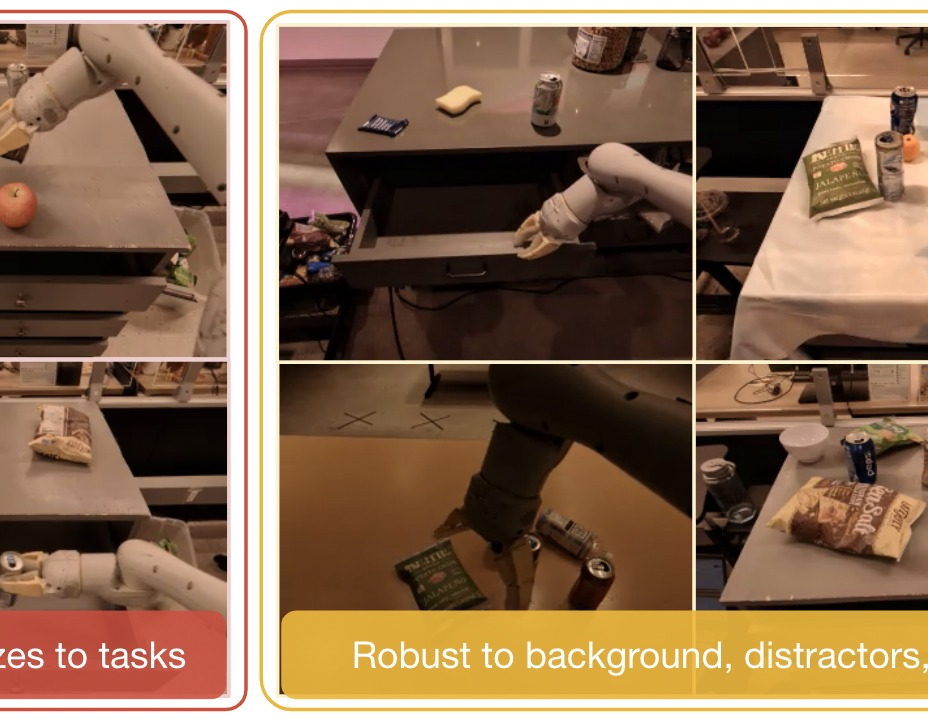
\includegraphics[width=1.803cm]{figures/img/canvas_tiles/col_301.jpg}}};
\draw[black!35,line width=0.35pt] (0.000,-1.280) rectangle (1.803,-2.687);
\node[anchor=north west,text=ACMDarkBlue,font=\tiny,inner sep=0] at (0.030,-2.707) {\href{https://arxiv.org/abs/2212.06817}{RT-1}};
\node[anchor=north west,inner sep=0] at (1.873,-1.280) {\href{https://arxiv.org/abs/2307.15818}{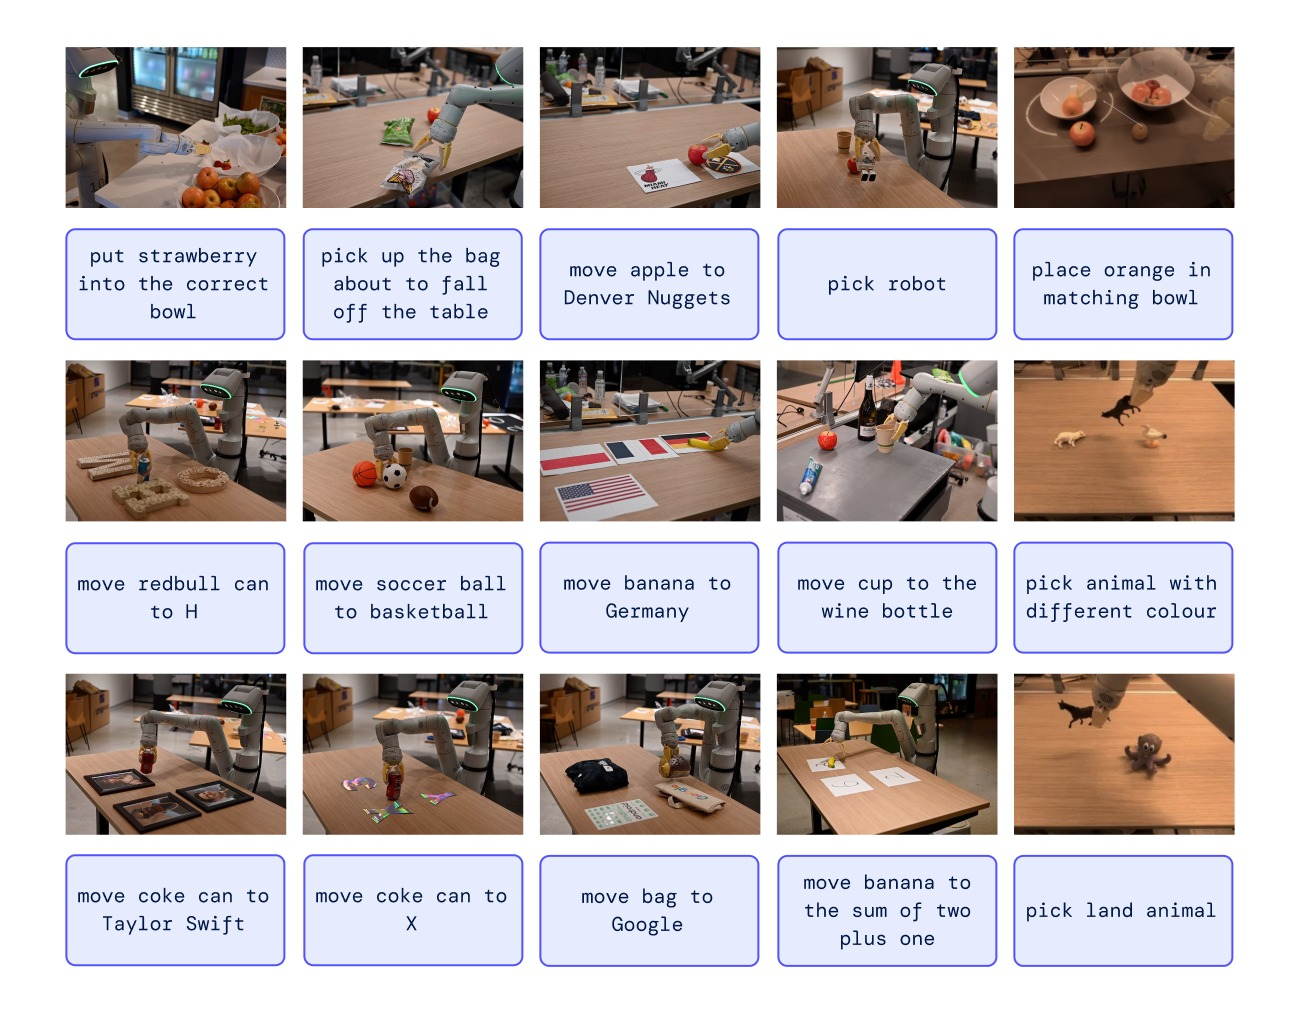
\includegraphics[width=1.803cm]{figures/img/canvas_tiles/col_303.jpg}}};
\draw[black!35,line width=0.35pt] (1.873,-1.280) rectangle (3.677,-2.687);
\node[anchor=north west,text=ACMDarkBlue,font=\tiny,inner sep=0] at (1.903,-2.707) {\href{https://arxiv.org/abs/2307.15818}{RT-2}};
\node[anchor=north west,inner sep=0] at (3.747,-1.280) {\href{https://arxiv.org/abs/2406.09246}{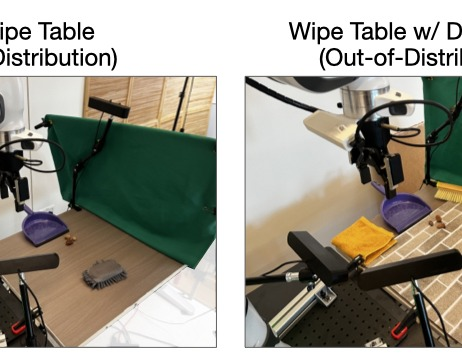
\includegraphics[width=1.803cm]{figures/img/canvas_tiles/col_204.jpg}}};
\draw[black!35,line width=0.35pt] (3.747,-1.280) rectangle (5.550,-2.687);
\node[anchor=north west,text=ACMDarkBlue,font=\tiny,inner sep=0] at (3.777,-2.707) {\href{https://arxiv.org/abs/2406.09246}{OpenVLA}};
\node[anchor=north west,inner sep=0] at (0.000,-3.057) {\href{https://arxiv.org/abs/2405.12213}{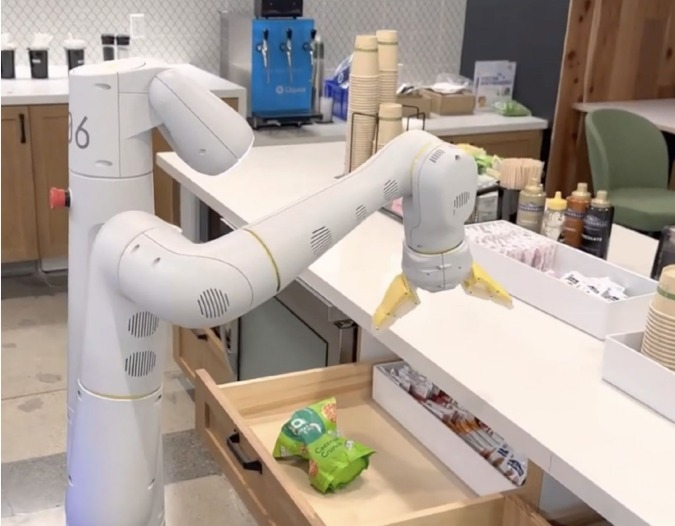
\includegraphics[width=1.803cm]{figures/img/canvas_tiles/col_189.jpg}}};
\draw[black!35,line width=0.35pt] (0.000,-3.057) rectangle (1.803,-4.463);
\node[anchor=north west,text=ACMDarkBlue,font=\tiny,inner sep=0] at (0.030,-4.483) {\href{https://arxiv.org/abs/2405.12213}{Octo}};
\node[anchor=north west,inner sep=0] at (1.873,-3.057) {\href{https://arxiv.org/abs/2410.24164}{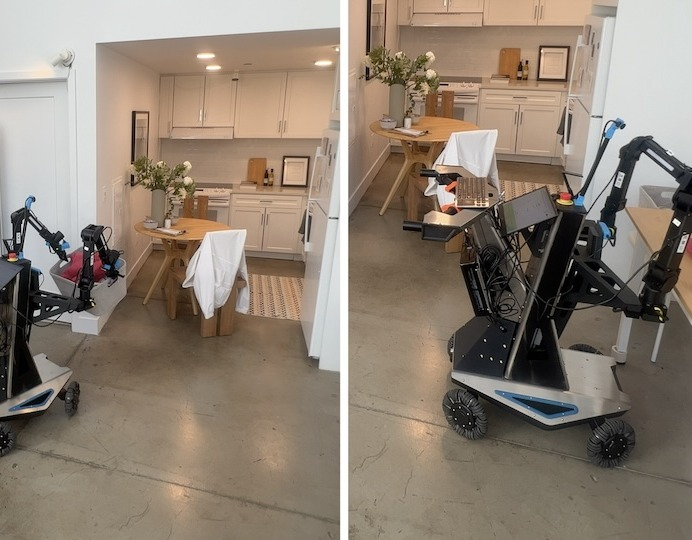
\includegraphics[width=1.803cm]{figures/img/canvas_tiles/col_218.jpg}}};
\draw[black!35,line width=0.35pt] (1.873,-3.057) rectangle (3.677,-4.463);
\node[anchor=north west,text=ACMDarkBlue,font=\tiny,inner sep=0] at (1.903,-4.483) {\href{https://arxiv.org/abs/2410.24164}{Pi-0}};
\node[anchor=north west,inner sep=0] at (3.747,-3.057) {\href{https://arxiv.org/abs/2411.19650}{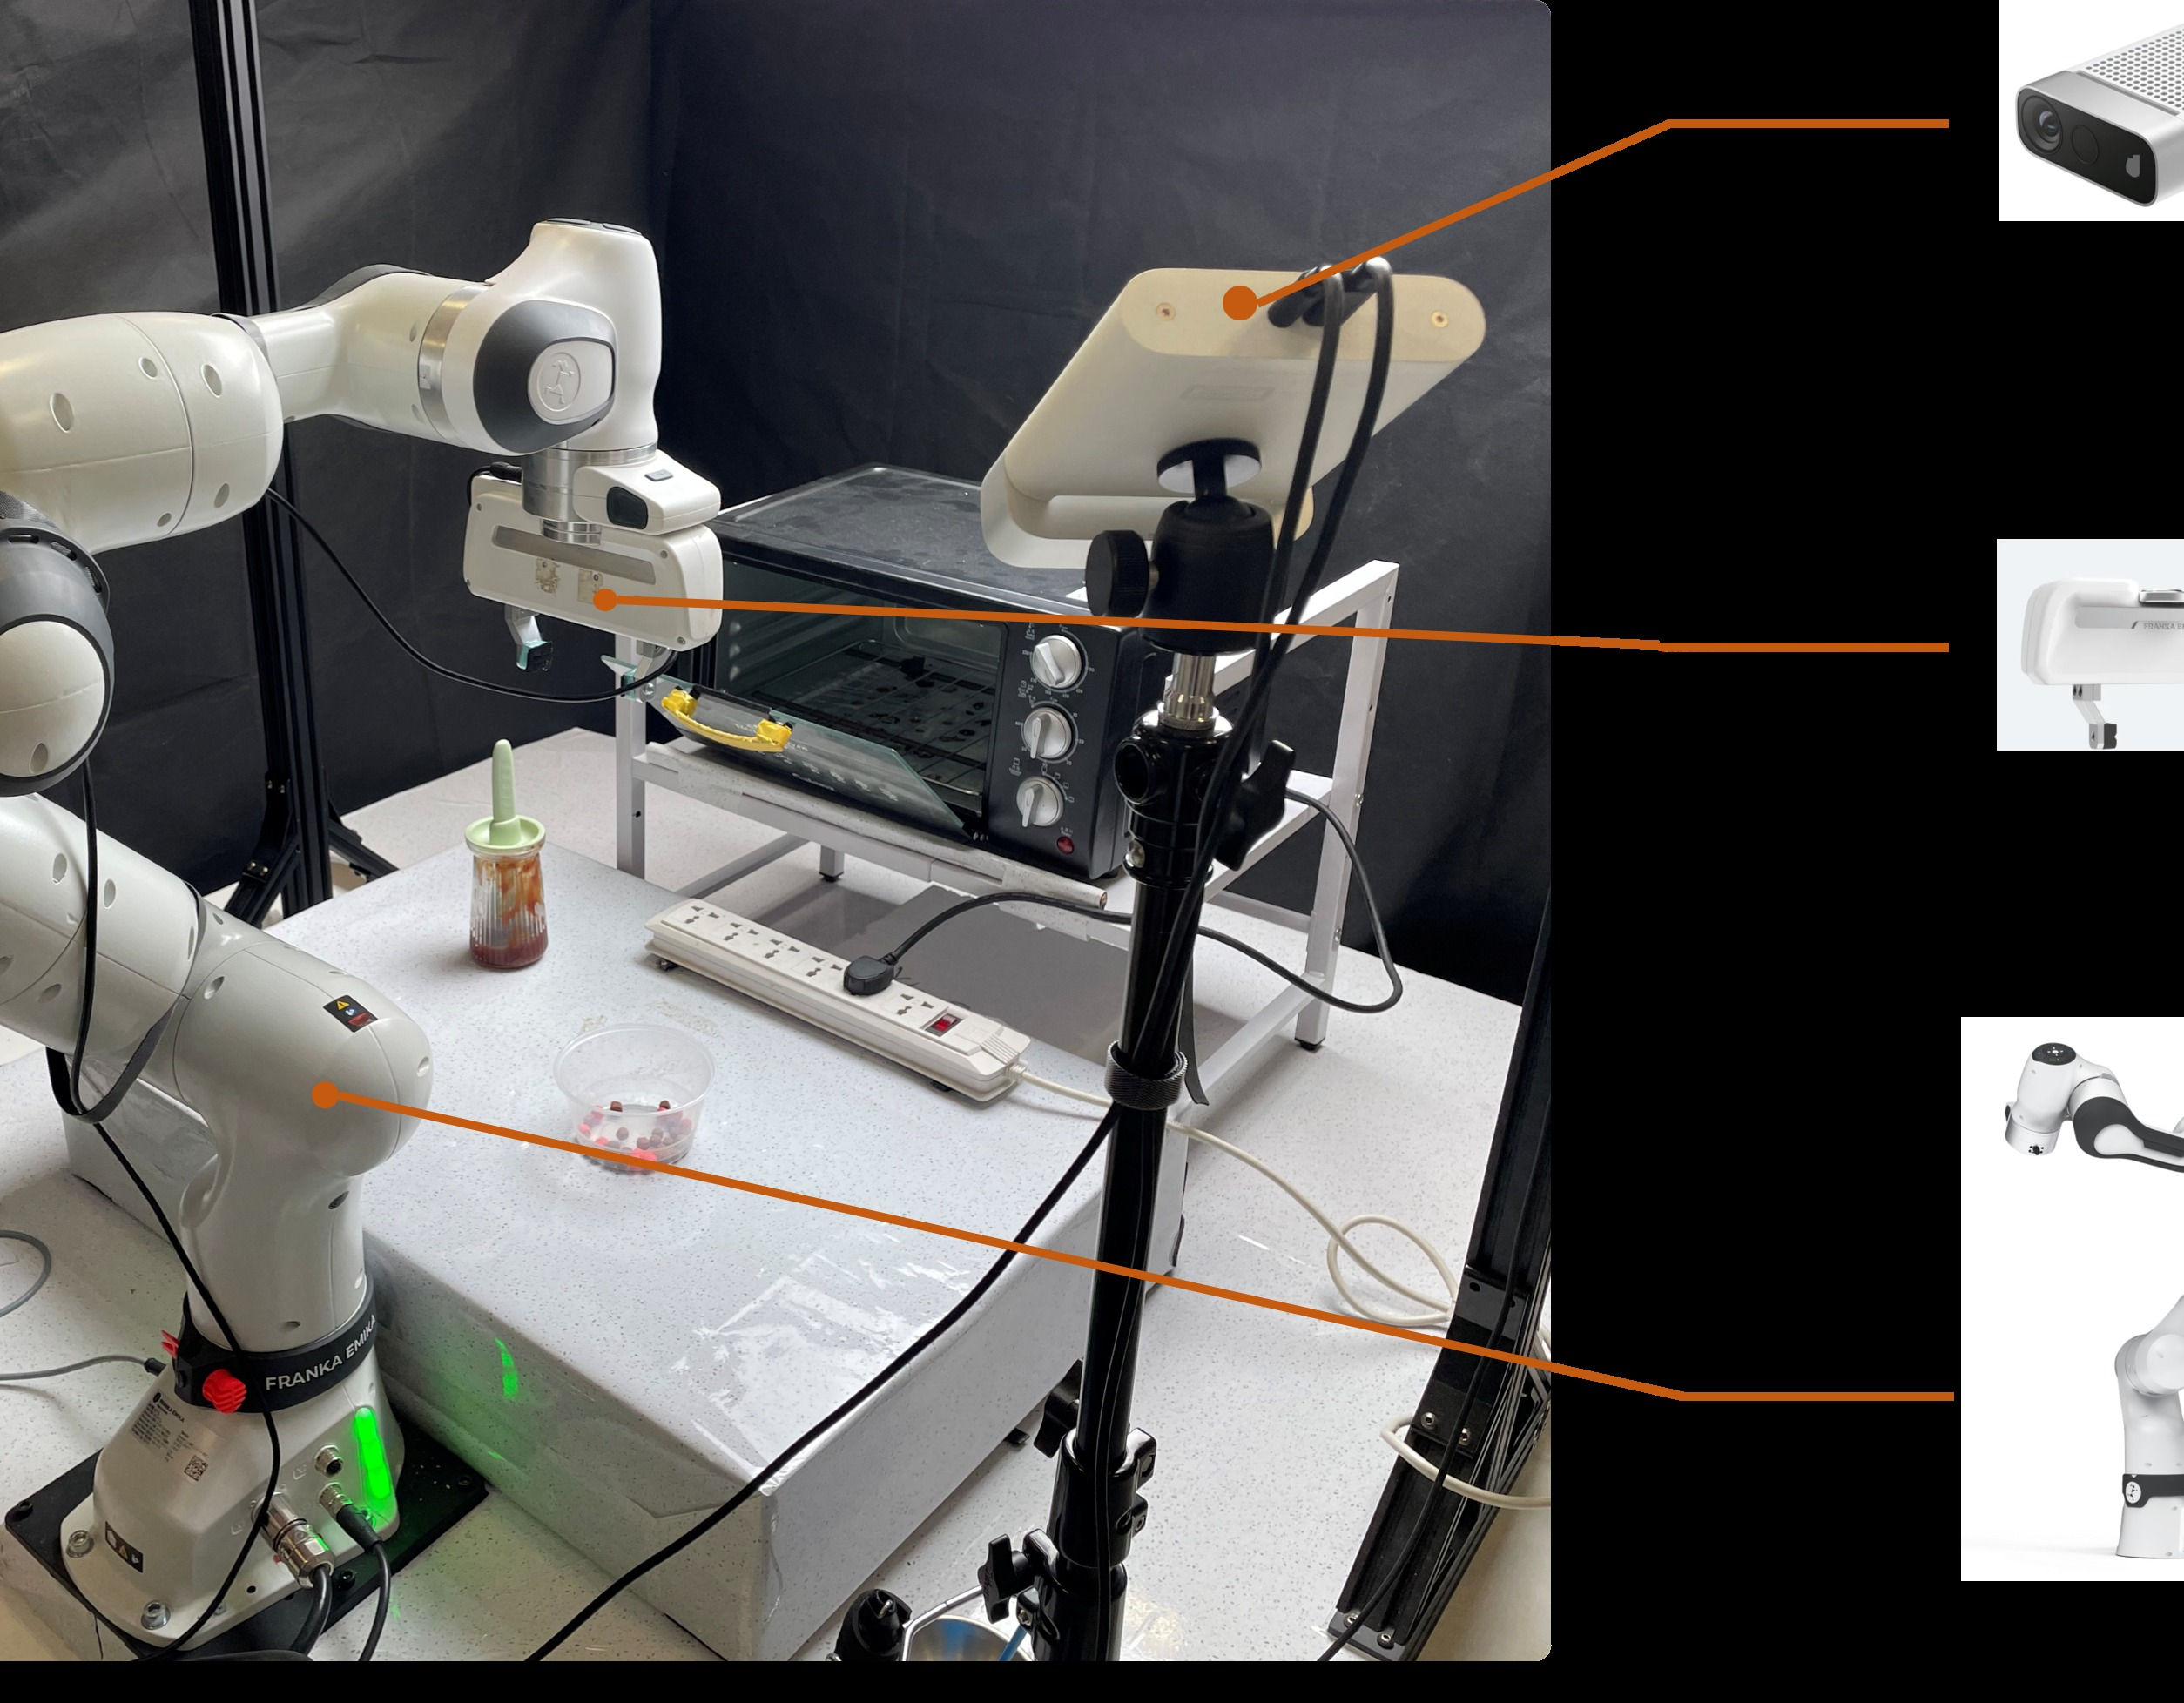
\includegraphics[width=1.803cm]{figures/img/canvas_tiles/col_50.jpg}}};
\draw[black!35,line width=0.35pt] (3.747,-3.057) rectangle (5.550,-4.463);
\node[anchor=north west,text=ACMDarkBlue,font=\tiny,inner sep=0] at (3.777,-4.483) {\href{https://arxiv.org/abs/2411.19650}{CogACT}};
\node[anchor=north west,inner sep=0] at (0.000,-4.833) {\href{https://arxiv.org/abs/2503.20020}{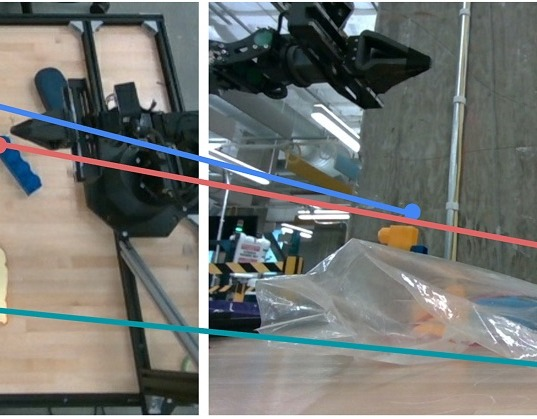
\includegraphics[width=1.803cm]{figures/img/canvas_tiles/col_115.jpg}}};
\draw[black!35,line width=0.35pt] (0.000,-4.833) rectangle (1.803,-6.240);
\node[anchor=north west,text=ACMDarkBlue,font=\tiny,inner sep=0] at (0.030,-6.260) {\href{https://arxiv.org/abs/2503.20020}{Gemini Robotics}};
\node[anchor=north west,inner sep=0] at (1.873,-4.833) {\href{https://arxiv.org/abs/2408.11812}{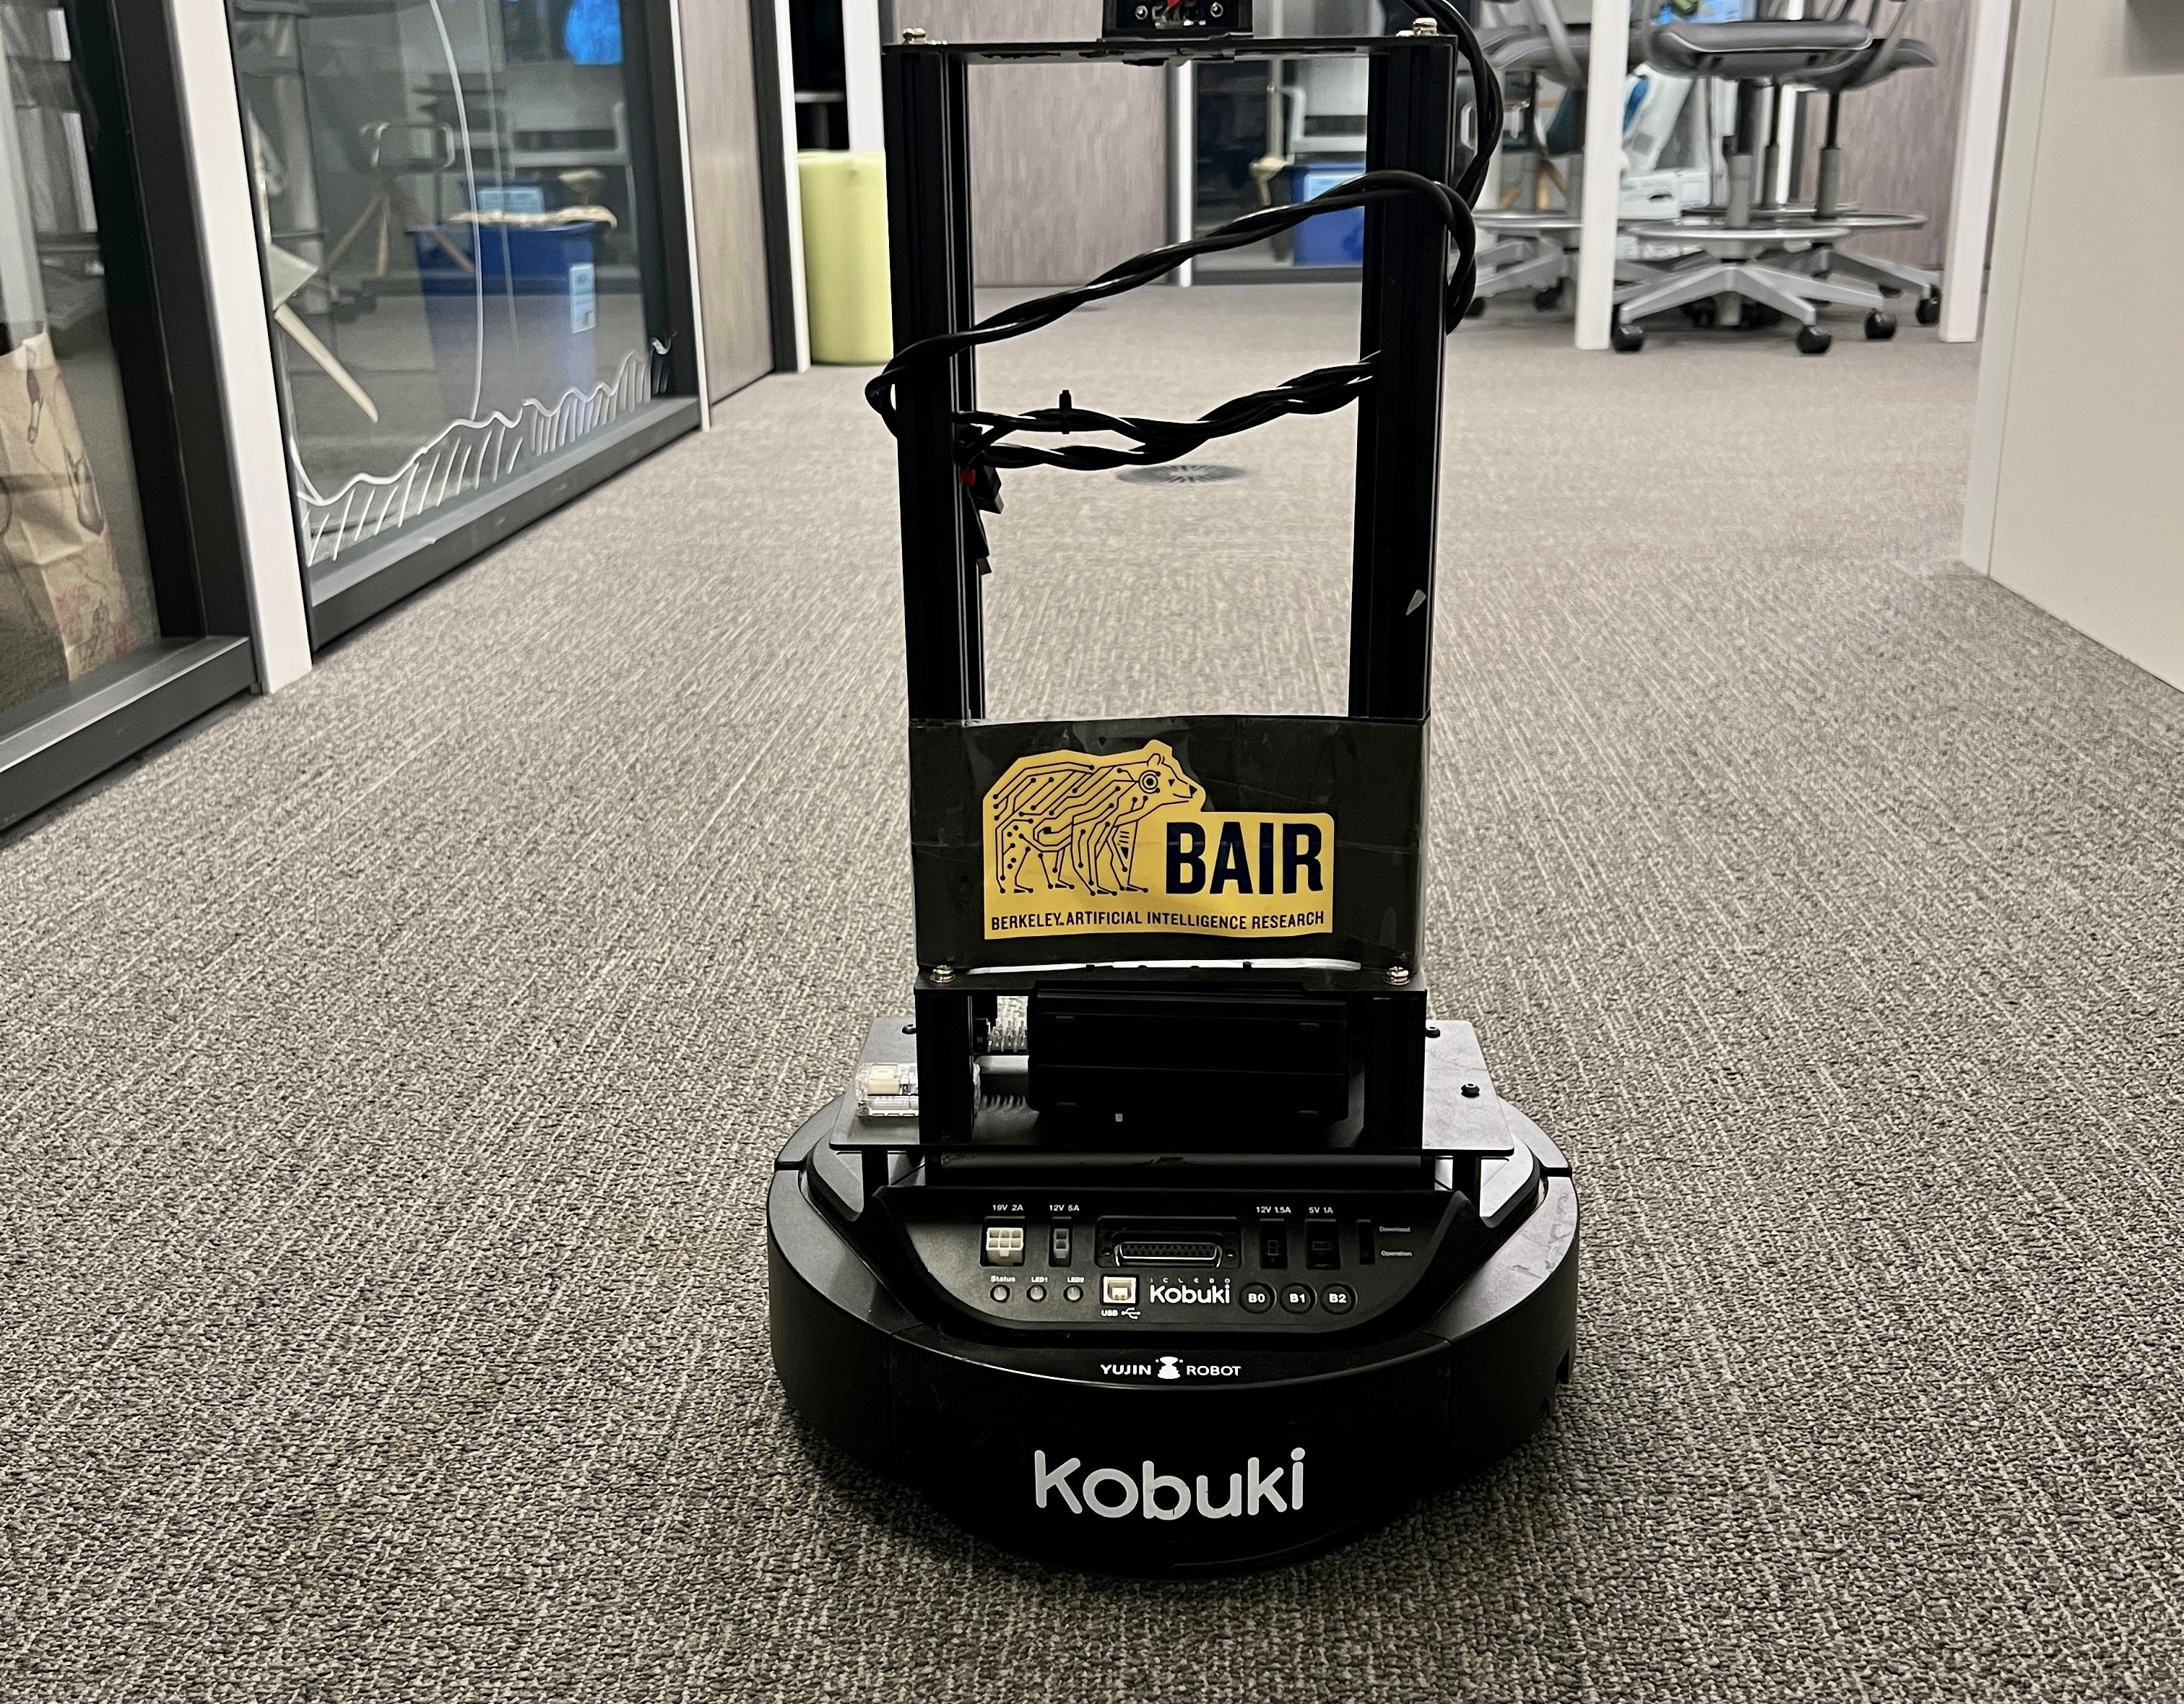
\includegraphics[width=1.803cm]{figures/img/canvas_tiles/col_56.jpg}}};
\draw[black!35,line width=0.35pt] (1.873,-4.833) rectangle (3.677,-6.240);
\node[anchor=north west,text=ACMDarkBlue,font=\tiny,inner sep=0] at (1.903,-6.260) {\href{https://arxiv.org/abs/2408.11812}{CrossFormer}};
\node[anchor=north west,inner sep=0] at (3.747,-4.833) {\href{https://arxiv.org/abs/2408.11812}{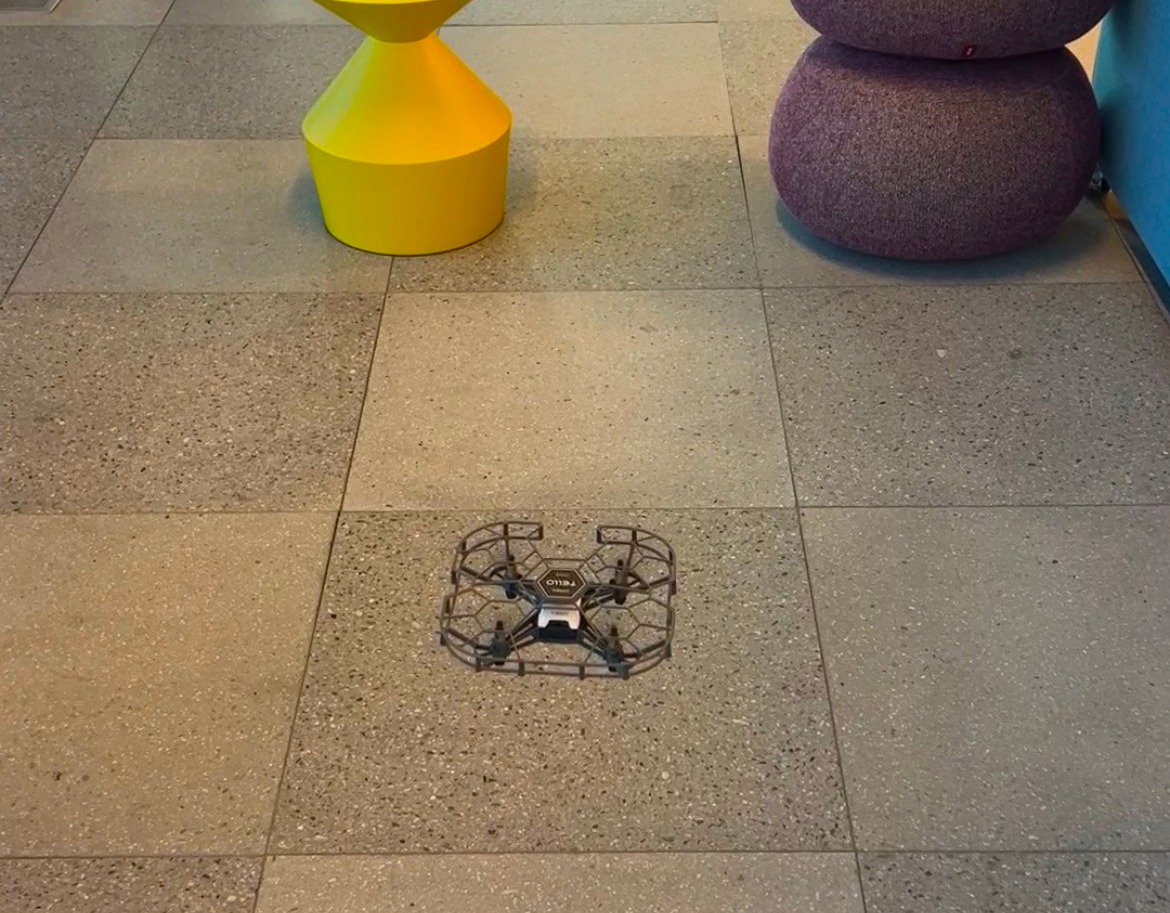
\includegraphics[width=1.803cm]{figures/img/canvas_tiles/col_55.jpg}}};
\draw[black!35,line width=0.35pt] (3.747,-4.833) rectangle (5.550,-6.240);
\node[anchor=north west,text=ACMDarkBlue,font=\tiny,inner sep=0] at (3.777,-6.260) {\href{https://arxiv.org/abs/2408.11812}{CrossFormer}};
\node[anchor=north west,inner sep=0] at (8.250,-1.280) {\href{https://arxiv.org/abs/2209.11302}{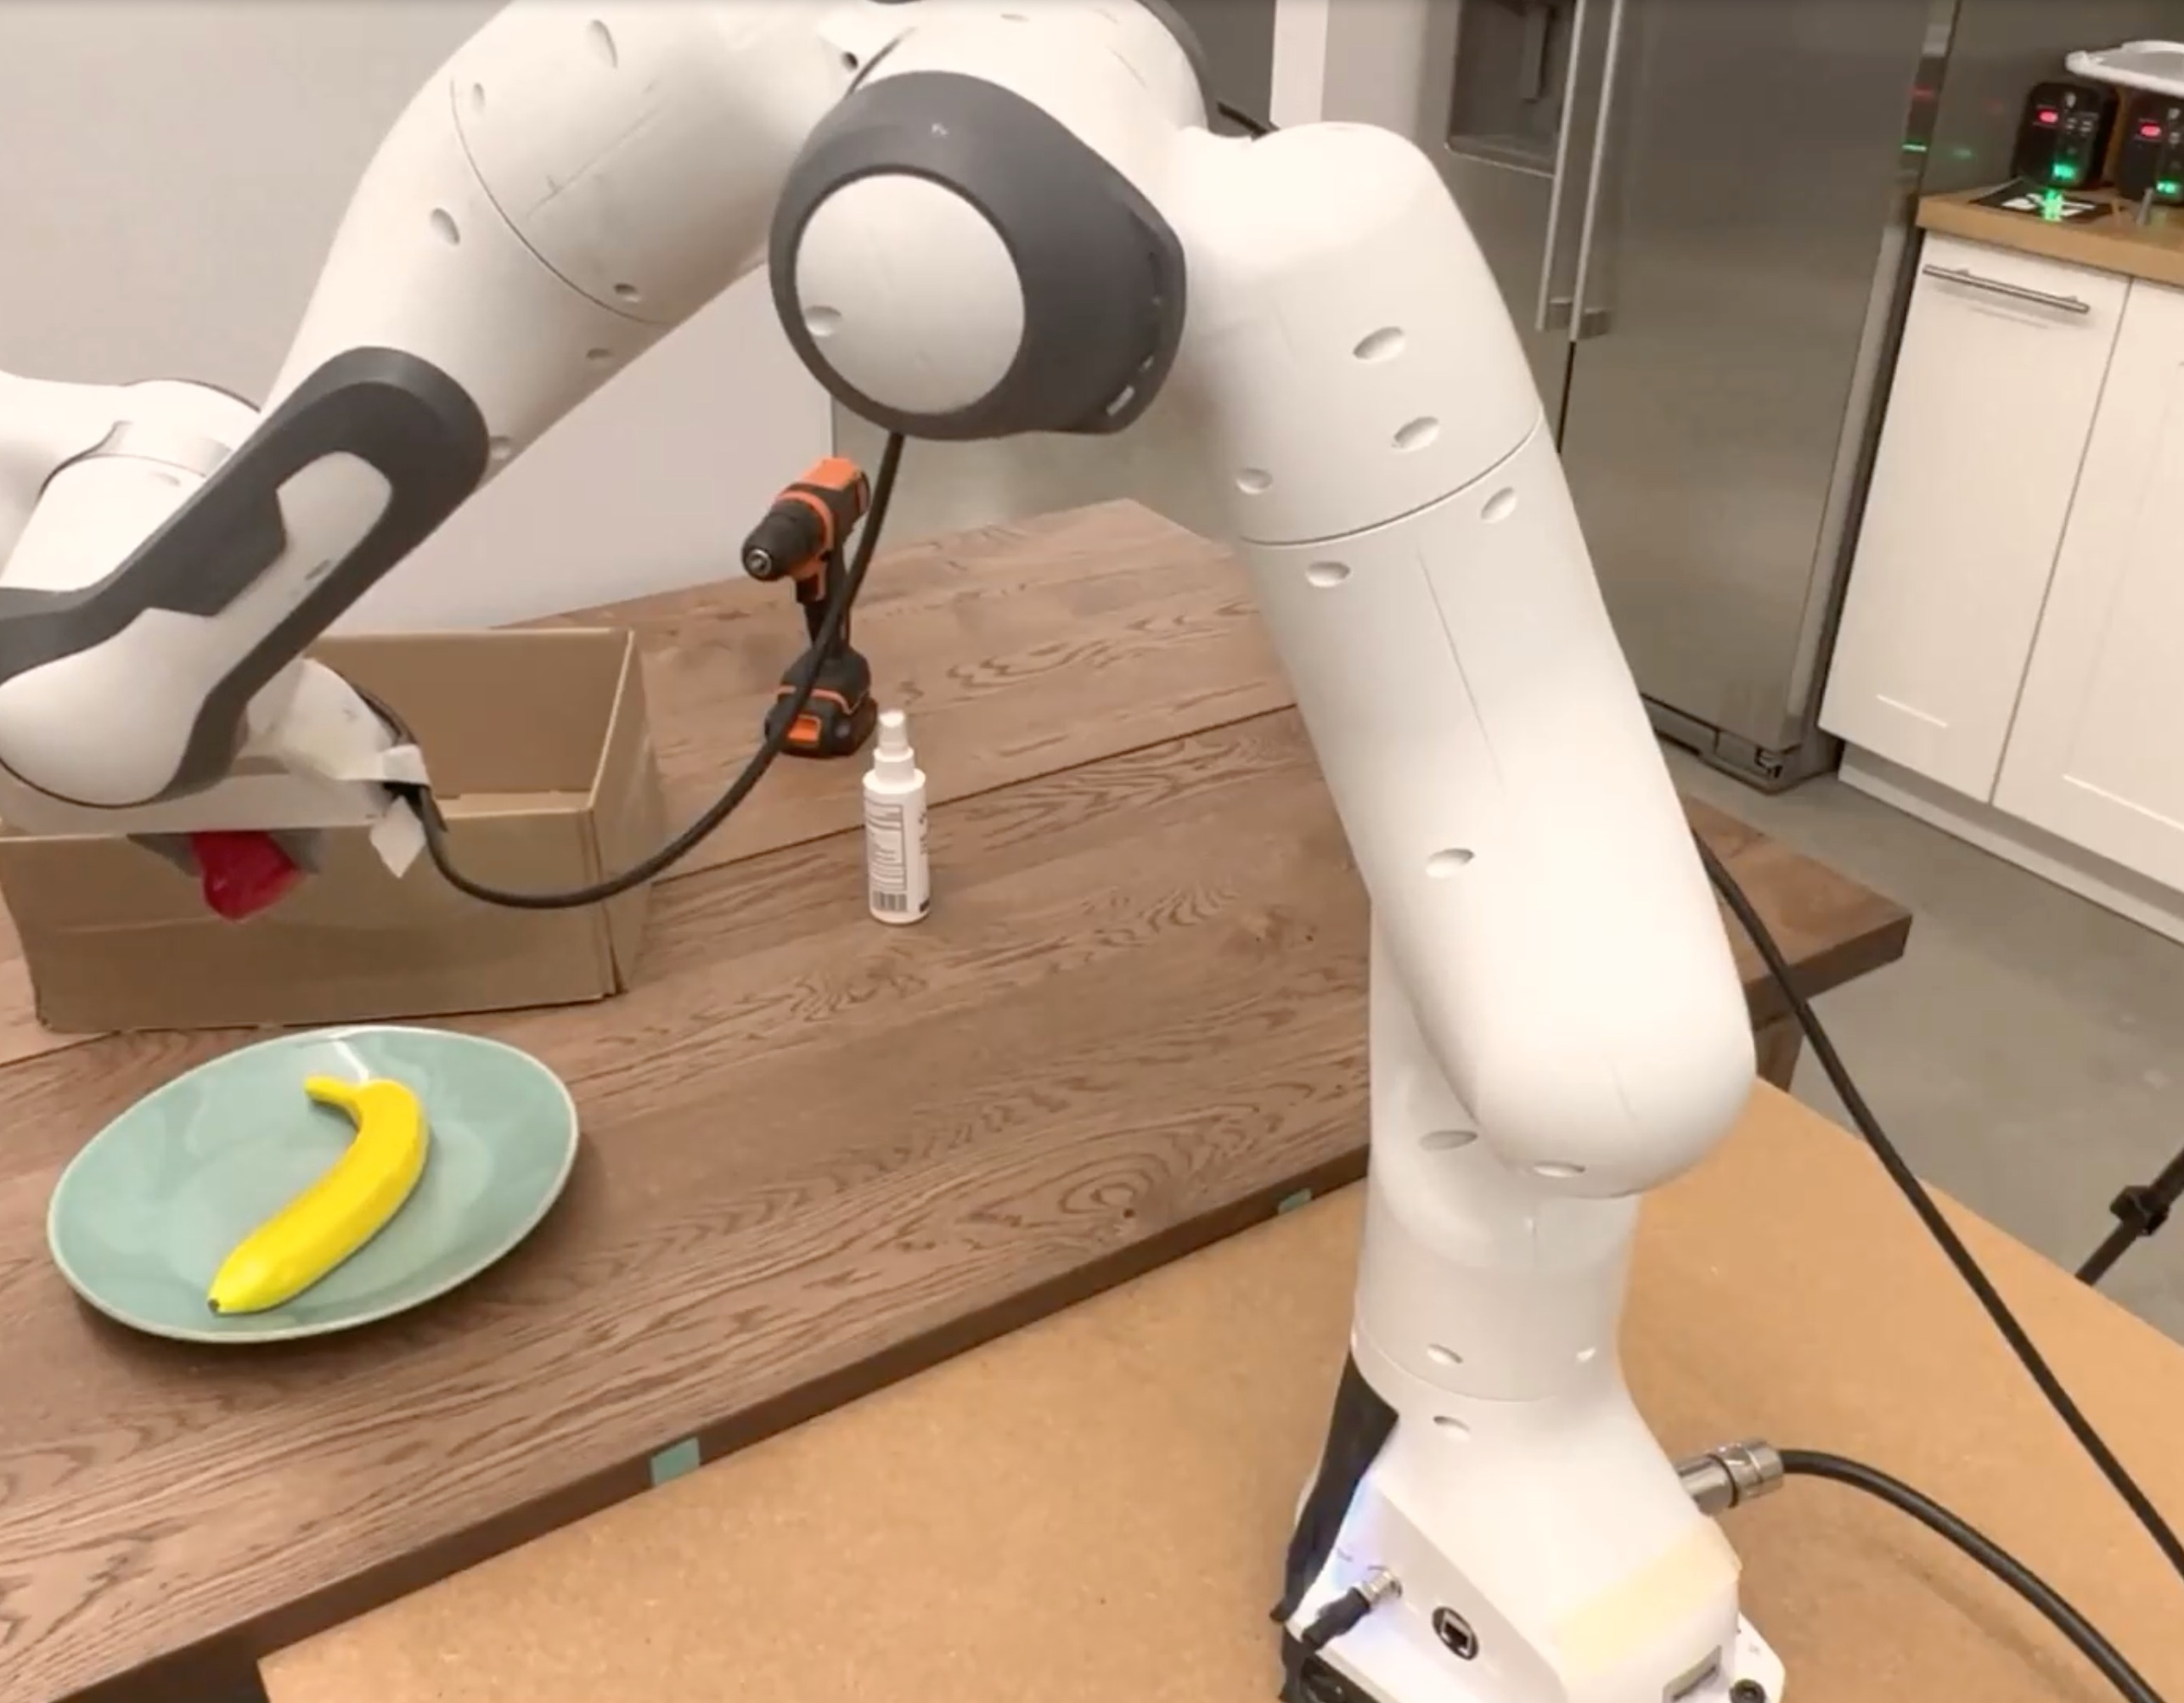
\includegraphics[width=1.803cm]{figures/img/canvas_tiles/col_226.jpg}}};
\draw[black!35,line width=0.35pt] (8.250,-1.280) rectangle (10.053,-2.687);
\node[anchor=north west,text=ACMDarkBlue,font=\tiny,inner sep=0] at (8.280,-2.707) {\href{https://arxiv.org/abs/2209.11302}{ProgPrompt}};
\node[anchor=north west,inner sep=0] at (10.123,-1.280) {\href{https://arxiv.org/abs/2307.05973}{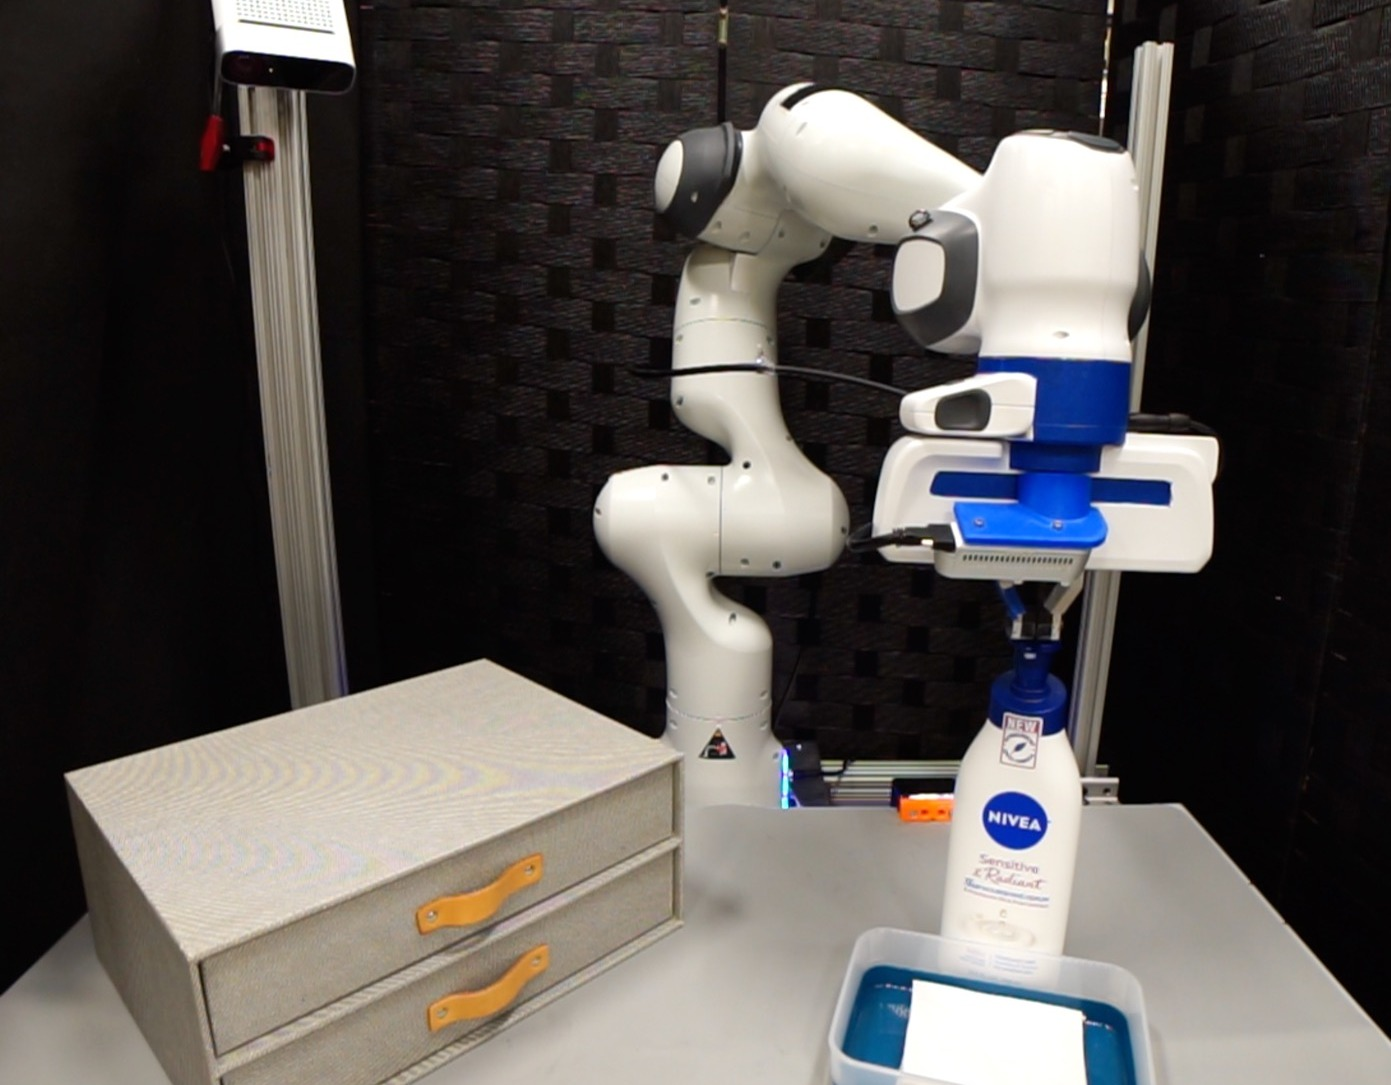
\includegraphics[width=1.803cm]{figures/img/canvas_tiles/col_351.jpg}}};
\draw[black!35,line width=0.35pt] (10.123,-1.280) rectangle (11.927,-2.687);
\node[anchor=north west,text=ACMDarkBlue,font=\tiny,inner sep=0] at (10.153,-2.707) {\href{https://arxiv.org/abs/2307.05973}{VoxPoser}};
\node[anchor=north west,inner sep=0] at (11.997,-1.280) {\href{https://arxiv.org/abs/2412.04455}{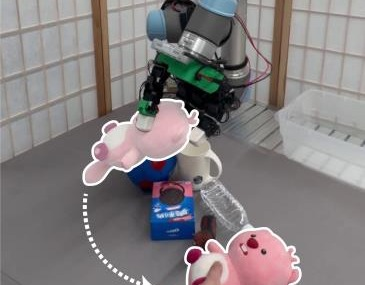
\includegraphics[width=1.803cm]{figures/img/canvas_tiles/col_40.jpg}}};
\draw[black!35,line width=0.35pt] (11.997,-1.280) rectangle (13.800,-2.687);
\node[anchor=north west,text=ACMDarkBlue,font=\tiny,inner sep=0] at (12.027,-2.707) {\href{https://arxiv.org/abs/2412.04455}{Code-as-Monitor}};
\node[anchor=north west,inner sep=0] at (8.250,-3.057) {\href{https://arxiv.org/abs/2306.15724}{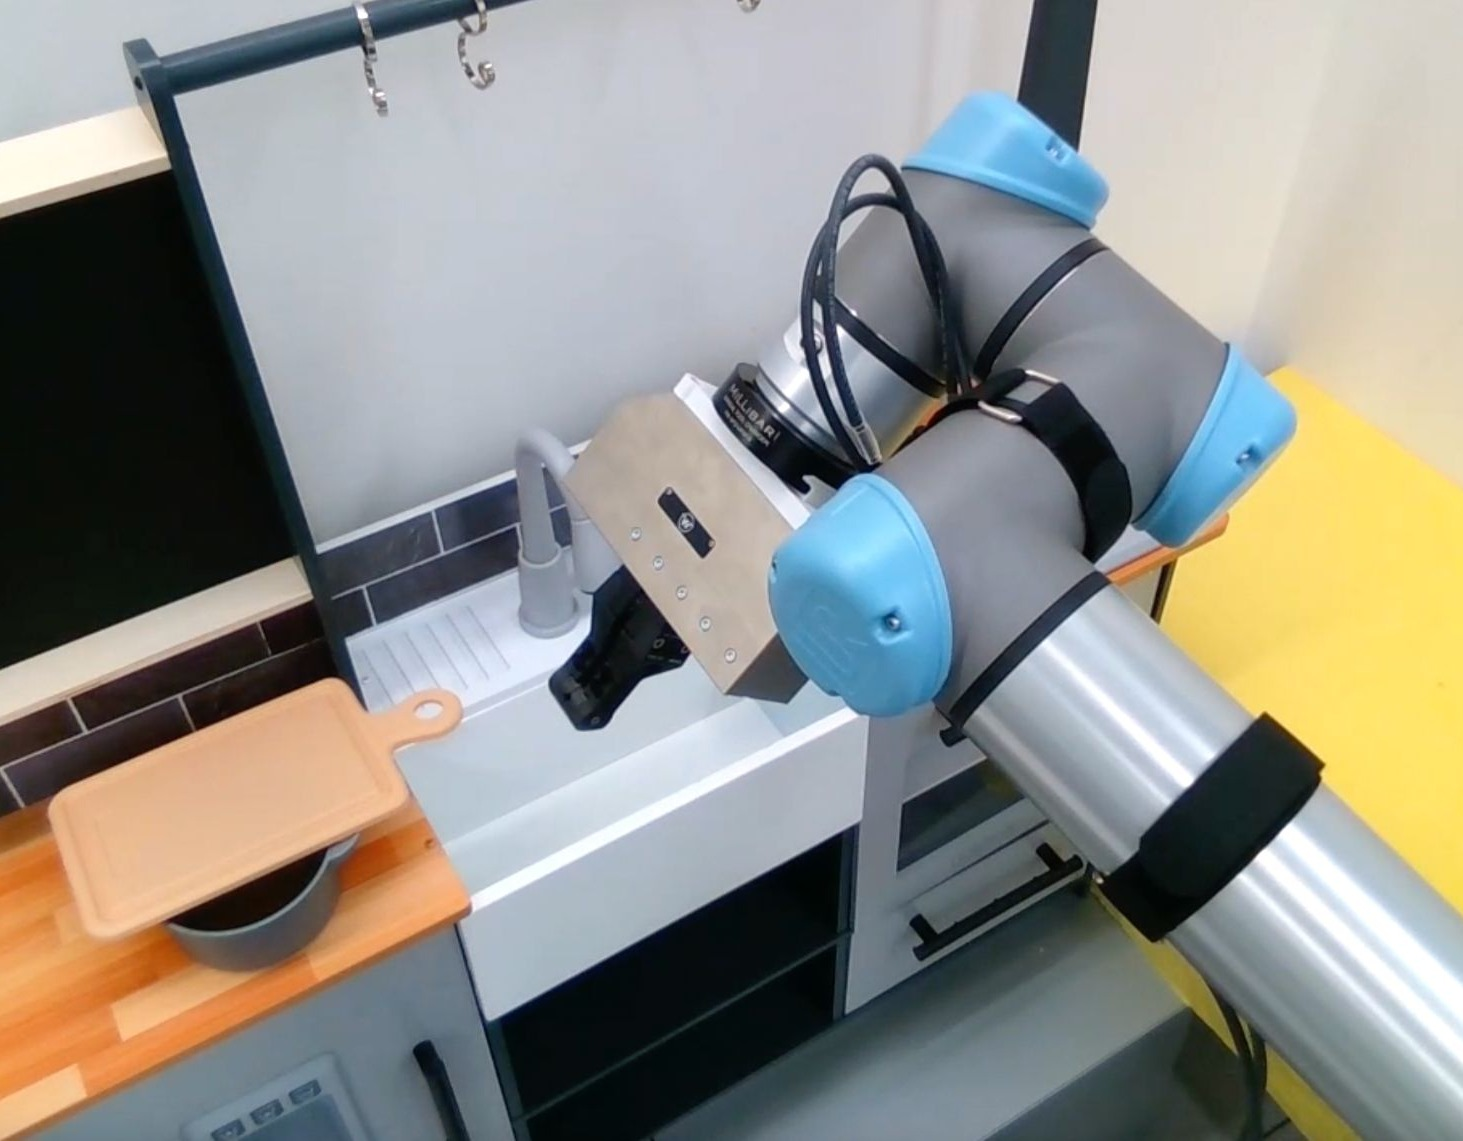
\includegraphics[width=1.803cm]{figures/img/canvas_tiles/col_240.jpg}}};
\draw[black!35,line width=0.35pt] (8.250,-3.057) rectangle (10.053,-4.463);
\node[anchor=north west,text=ACMDarkBlue,font=\tiny,inner sep=0] at (8.280,-4.483) {\href{https://arxiv.org/abs/2306.15724}{REFLECT}};
\node[anchor=north west,inner sep=0] at (10.123,-3.057) {\href{https://arxiv.org/abs/2305.05658}{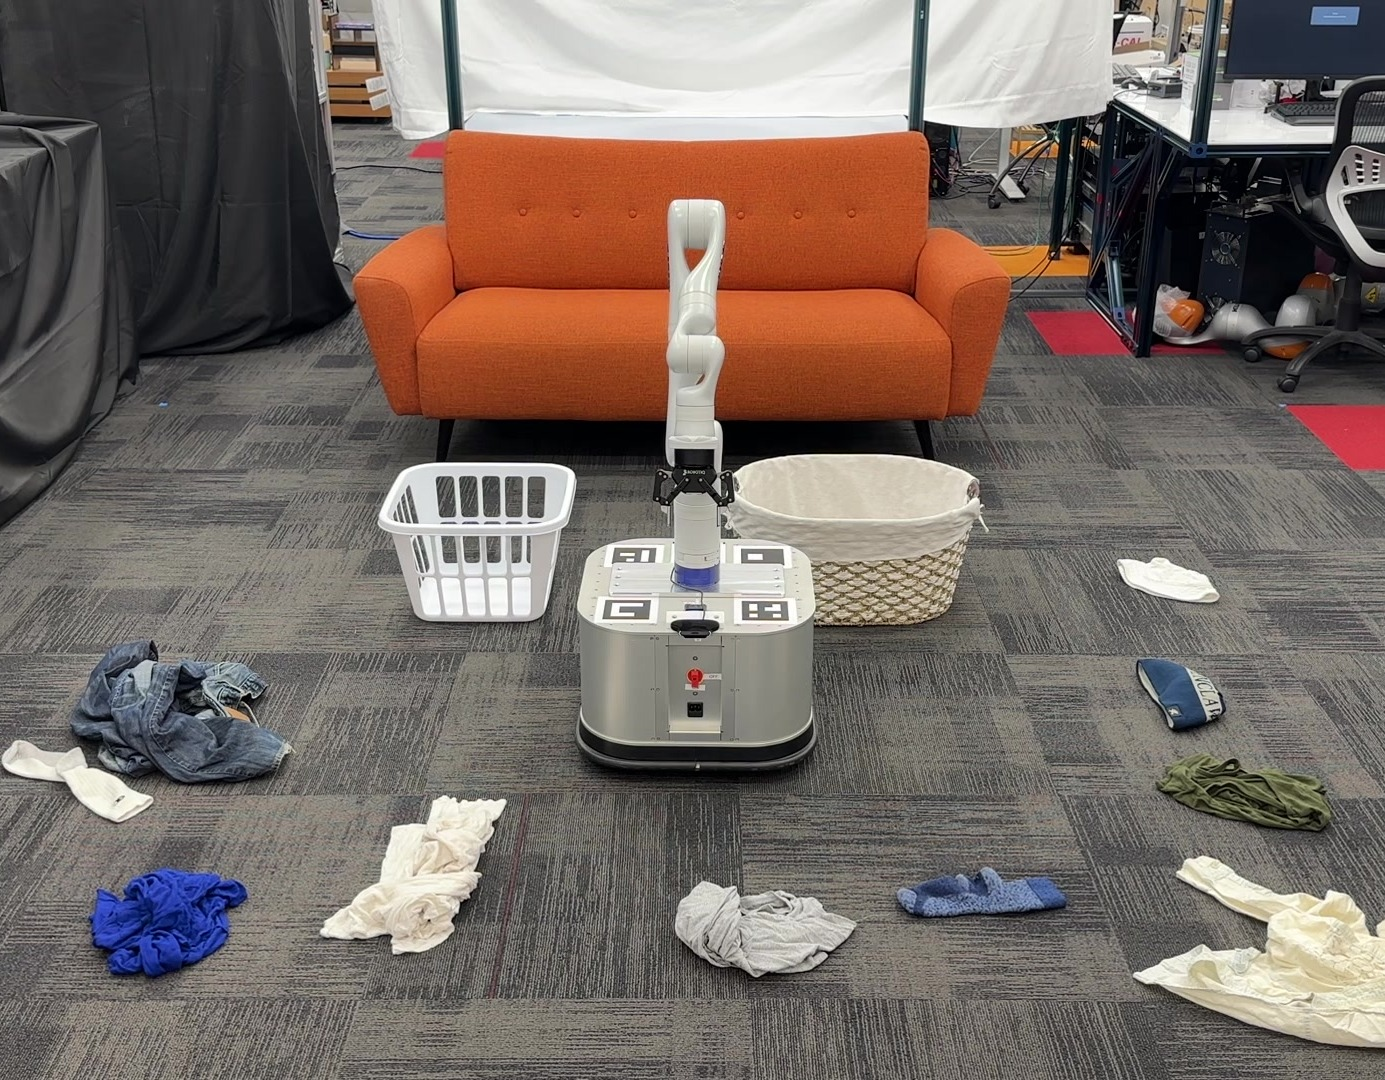
\includegraphics[width=1.803cm]{figures/img/canvas_tiles/col_338.jpg}}};
\draw[black!35,line width=0.35pt] (10.123,-3.057) rectangle (11.927,-4.463);
\node[anchor=north west,text=ACMDarkBlue,font=\tiny,inner sep=0] at (10.153,-4.483) {\href{https://arxiv.org/abs/2305.05658}{TidyBot}};
\node[anchor=north west,inner sep=0] at (11.997,-3.057) {\href{https://arxiv.org/abs/2305.11176}{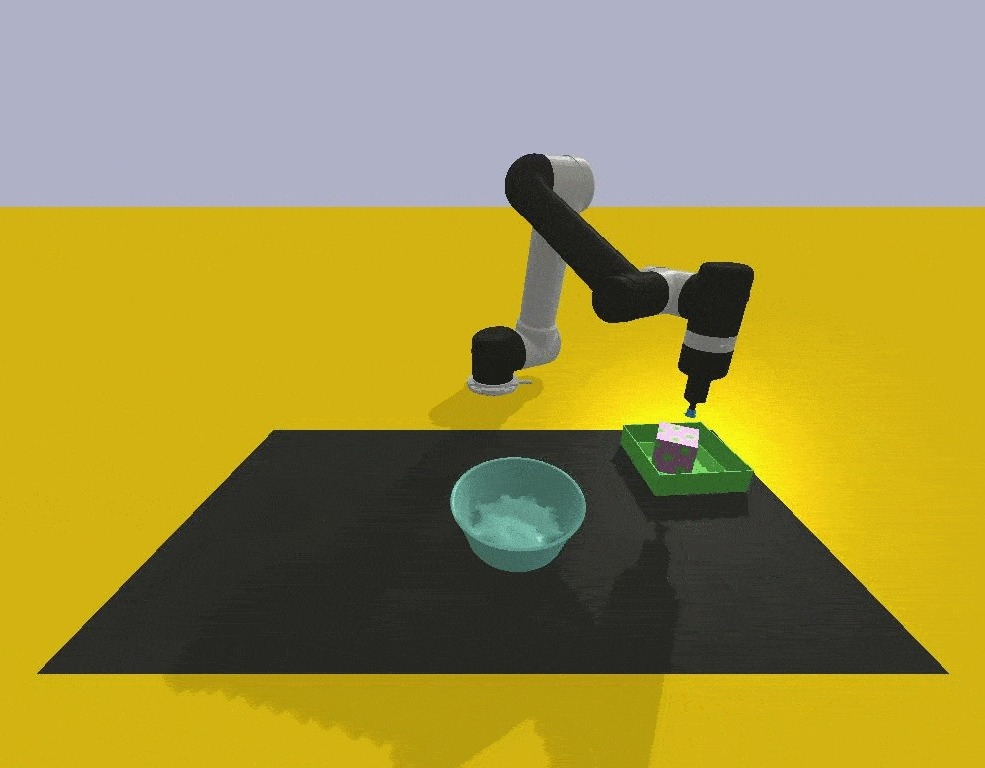
\includegraphics[width=1.803cm]{figures/img/canvas_tiles/col_128.jpg}}};
\draw[black!35,line width=0.35pt] (11.997,-3.057) rectangle (13.800,-4.463);
\node[anchor=north west,text=ACMDarkBlue,font=\tiny,inner sep=0] at (12.027,-4.483) {\href{https://arxiv.org/abs/2305.11176}{Instruct2Act}};
\node[anchor=north west,inner sep=0] at (8.250,-4.833) {\href{https://arxiv.org/abs/2309.09969}{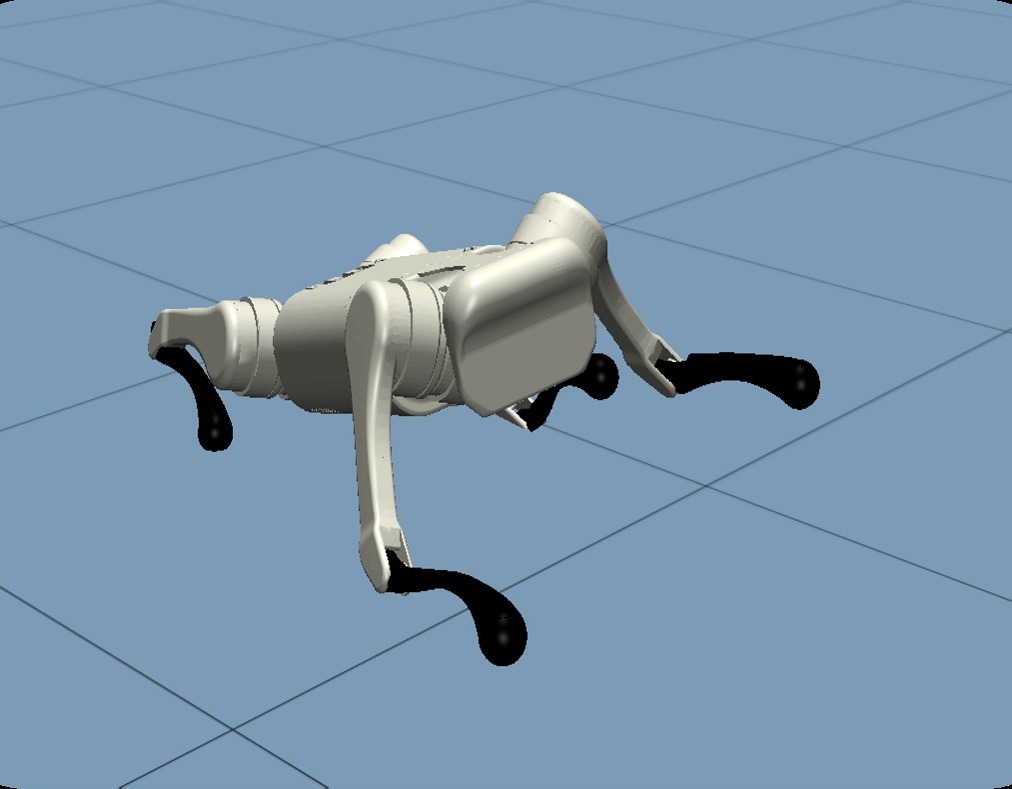
\includegraphics[width=1.803cm]{figures/img/canvas_tiles/col_232.jpg}}};
\draw[black!35,line width=0.35pt] (8.250,-4.833) rectangle (10.053,-6.240);
\node[anchor=north west,text=ACMDarkBlue,font=\tiny,inner sep=0] at (8.280,-6.260) {\href{https://arxiv.org/abs/2309.09969}{Prompt2Walk}};
\node[anchor=north west,inner sep=0] at (10.123,-4.833) {\href{https://arxiv.org/abs/2307.00329v3}{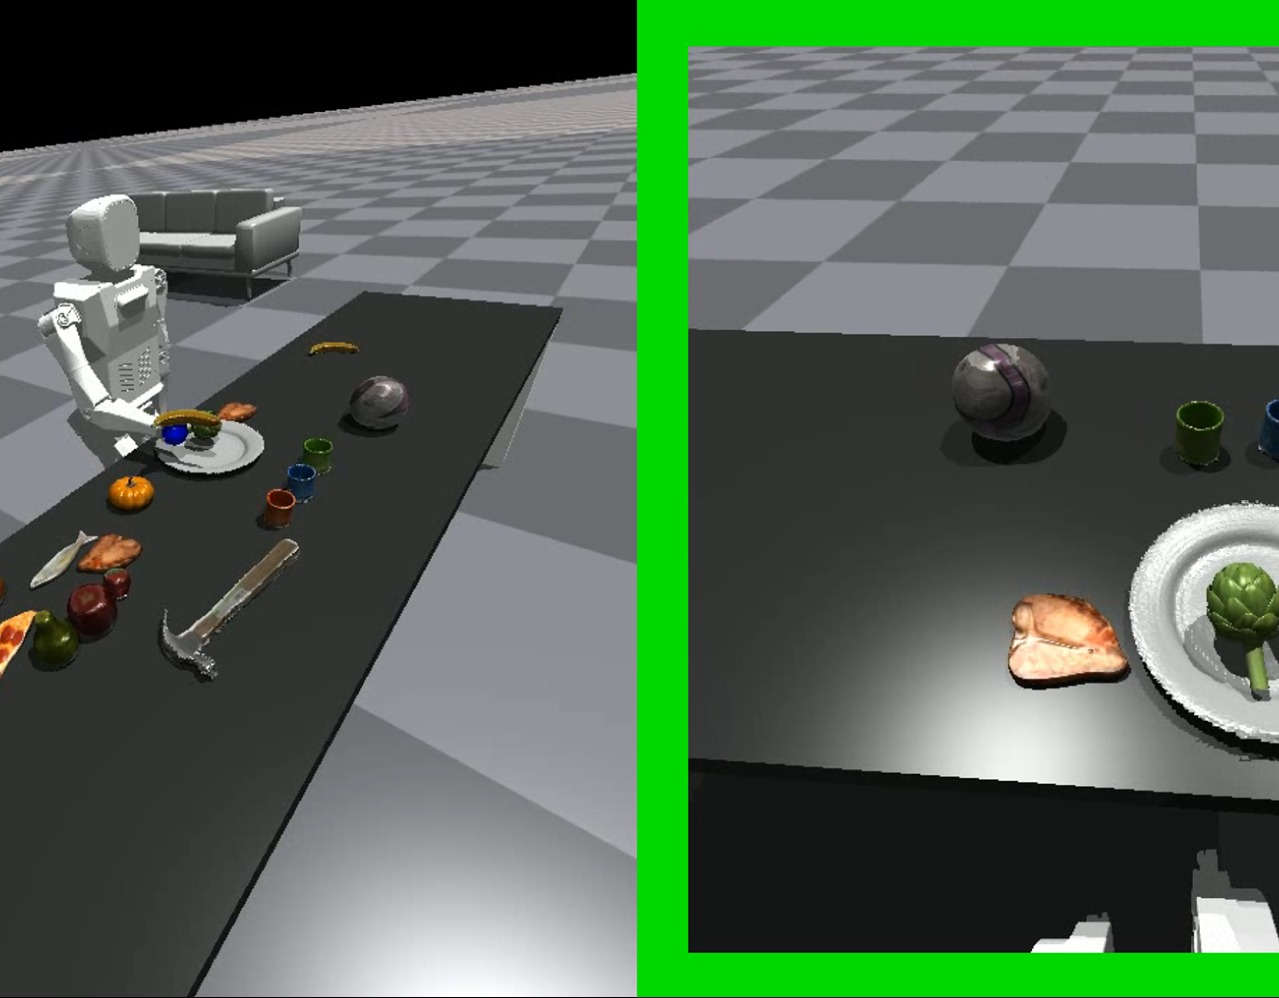
\includegraphics[width=1.803cm]{figures/img/canvas_tiles/col_73.jpg}}};
\draw[black!35,line width=0.35pt] (10.123,-4.833) rectangle (11.927,-6.240);
\node[anchor=north west,text=ACMDarkBlue,font=\tiny,inner sep=0] at (10.153,-6.260) {\href{https://arxiv.org/abs/2307.00329v3}{DoReMi}};
\node[anchor=north west,inner sep=0] at (11.997,-4.833) {\href{https://arxiv.org/abs/2603.22435}{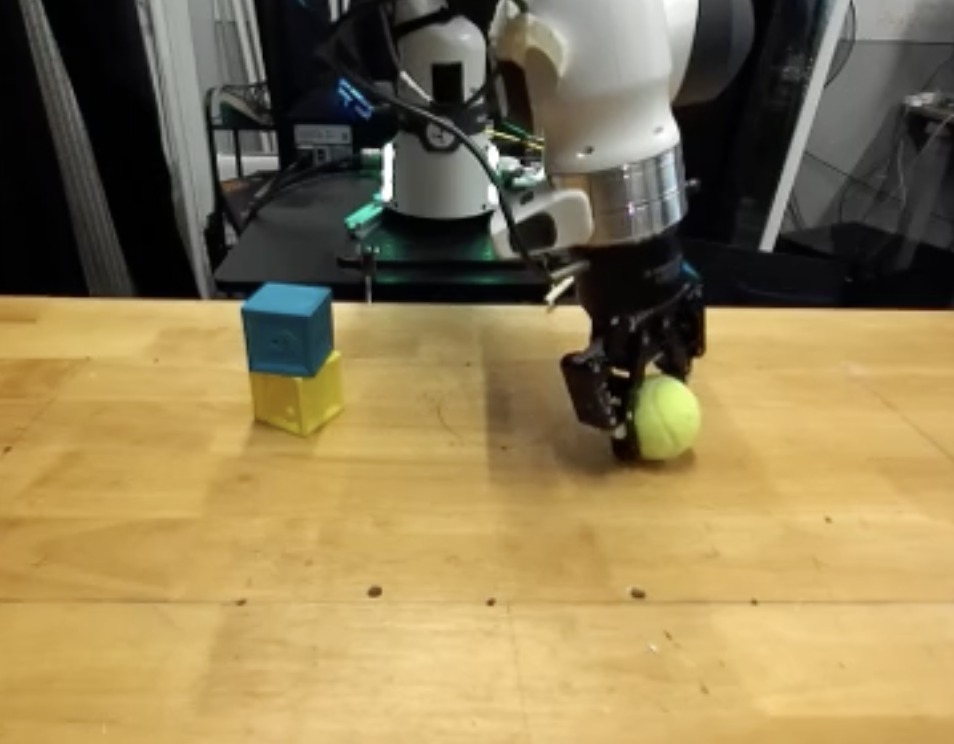
\includegraphics[width=1.803cm]{figures/img/canvas_tiles/col_27.jpg}}};
\draw[black!35,line width=0.35pt] (11.997,-4.833) rectangle (13.800,-6.240);
\node[anchor=north west,text=ACMDarkBlue,font=\tiny,inner sep=0] at (12.027,-6.260) {\href{https://arxiv.org/abs/2603.22435}{CaP-X}};
\end{tikzpicture}}
\caption{\textbf{Weights or Skills?} The survey's organising question, posed with real systems. \emph{Weights} (left): vision-language-action policies ship frozen network weights that map observations to actions (\S\ref{sec:vla}). \emph{Skills} (right): code-as-policy agents ship executable programs and improve them from their own experience (\S\ref{sec:code}). The 77 taxonomy systems populate these two poles across six technique branches (2016--2026). Every photo is a hyperlink to its source paper; per-panel provenance is in Table~\ref{tab:canvas_provenance}. Images \textcopyright\ their respective authors, reproduced for scholarly review.}
\Description{Two panels of robot photographs posing the survey's central dichotomy. Left, labelled WEIGHTS: vision-language-action systems (RT-1, RT-2, OpenVLA, Octo, Pi-0, CogACT, Gemini Robotics, CrossFormer). Right, labelled SKILLS: code-as-policy systems (ProgPrompt, VoxPoser, Code-as-Monitor, REFLECT, TidyBot, Instruct2Act, Prompt2Walk, DoReMi, CaP-X). A central spine reads 'what ships? frozen network weights vs executable programs'.}
\label{fig:corpus_collage}
\end{figure*}
